% Appendix A

\chapter{Batches fabrication and hardness/density measurements details} % Main appendix title

\label{AppendixA} % For referencing this appendix elsewhere, use \ref{AppendixA}

\section{Process parameters and measured hardness/density properties}
\label{ppa}
All manufacturing set values are gathered in table \ref{table:Pparam}. Dimensions of the cubic, cylindrical and parallelepiped specimens are noted in accordance with figure \ref{fig:cc}.\\

 \begin{center}
%\begin{table}[ht]
\setlength\LTleft{-0.7in}
%\setlength\LTright{-1in}
\begin{landscape}
\begin{savenotes}

\begin{longtable}{@{\extracolsep{\fill}}*{12}{|c}|@{}}
    \hline
  Batch name & Contour & Type & Dimensions [mm] &Specimen name & $\frac{P}{P_{max}} [-]$ & $v_s [\frac{mm}{s}]$ & $E_d [\frac{J}{mm^3}]$ & $H_v [HV]$ & $\rho_{rel}$ \footnote{Measured by RODIA [\%].} & $\rho_{a,rel}$ \footnote{Measured by HW (AB specimens) [\%].} & $\rho_{a,rel}$ \footnote{Measured by HW (polished specimens) [\%].} \\
  \hline
  \hline
  \endfirsthead
\multicolumn{12}{c}%
{\tablename\ \thetable\ -- \textit{Continued from previous page}} \\
\hline
Batch name & Contour & Type & Dimensions [mm] &Specimen name & $\frac{P}{P_{max}} [-]$ & $v_s [\frac{mm}{s}]$  & $E_d [\frac{J}{mm^3}]$ & $H_v [HV]$ & $\rho_{rel}$  & $\rho_{a,rel}$  & $\rho_{a,rel}$ \\
\hline
\endhead

\hline \multicolumn{12}{c}{\textit{Continued on next page}} \\
\caption[Manufacturing process parameters]{Manufacturing process parameters}
\label{table:Pparam}

\endfoot
\hline
\endlastfoot

  X200-171024 & No & Cubic & L=10& 1 & 0.85 & 900 & 86.13 &135.9 & - &99.24 &-\\
  & &   & & 2 &  & 1000 & 77.52 &133.7 &- &99.08 &-\\
  & &   & & 3&  & 1059& 73.20 &135.5 & -&99.00 &-\\
  & &  & & 4&  & 1500&51.68 &137.3 & -&99.38 &-\\
  & &  & & 5& 1 & 900&101.33 &131.3 &- &98.81 &-\\
  & &  & & 6&  & 1059&86.12 &132.7 & -&98.83 &-\\
  & & & & 7 & 0.75 & 1200& 57 &137.3 &- &99.49 &-\\
  & & & & 7a & & & &137.9 & -&99.33 &-\\
  & & & & 7b & & & &137.9 &- &99.45 &-\\
  & & & & 8& & 900&76 &135.5 &- &99.23 &-\\
    & & & & 8a & & & & 133.7& -&98.77 &-\\
      & & & & 8b & & & & 136.1& -&99.23 &-\\
\hline  
  X200-180109 & No&Cubic & L=10 & 7c & 0.75 &1200 &57 &141.0 &99.77 &99.33 &99.77\\
  & & & & 7d & && &138.6  &- &99.45 &-\\
  & & & & 7e & & & &140.0 &- &99.44 & -\\
    & & & & 7n & & & &141.4 &- &99.45 &-\\
  & & & & 7g & & & &139.4 & -&99.50 &-\\
  & & & & 7h & & & &139.2 &99.51 &99.52 &99.32\\ 
  & & & & 7i & & & &140.3 &- &99.48 &-\\        
  & & & & 7j & & & &140.9 & -&99.48 &-\\        
  & & & & 7k & & & &140.6 & -&99.37 &-\\        
  & & & & 7l & & & &139.8 & -&99.38 &-\\        
  & & & & 7m & & & &139.0 &99.65 &99.29 &99.48\\      
  & & & & 7n & & & &140.0 &99.51 &99.24 &99.48\\      
  & & & & 7o & & & &138.7 &99.52 &99.49 &99.49\\
  & & & & 7p & & & &140.6 & -&99.37 &-\\
  & & & & 7q & & & &139.0 & -&99.31 &-\\                    
  & & & & 8c& & 900 & 76 &139.4 &- &99.27 &-\\
  & & & & 8d & & & &138.8 & -&99.20 &-\\
  & & & & 8e & & & &138.0 &- &99.29 &-\\
  & & & & 8f & & & &138.3 & -&99.50 &-\\
  & & & & 8g & & & &138.2 & -&99.37 &-\\
  & & & & 8h & & & &139.5 & -&99.51 &-\\
  & & & & 8i & & & &134.6 &- &99.18 &-\\
  & & & & 8j & & & &138.0 & -&99.44 &-\\
  & & & & 8k & & & &138.0 &- &99.41 &-\\  
  & & & & 8l & & & &136.5 & -&99.39 &-\\
  & & & & 8m & & & &139.0 & -&99.31 &-\\
  & & & & 8n & & & &140.4 &- &99.29 &-\\
  & & & & 8o & & & &138.5 &- &99.54 &-\\     
  & & & & 8p & & & &138.7 & -&99.35 &-\\
  & & & & 8q & & & &138.7 & -&99.43 &-\\        
\hline  
  X200-180220 & No & Cubic & L=5 & TT150-2 & 0.75 & 1200 & 57 & & -  & -&-\\
  & &  & & TT200-2 &  & & & &- & -&-\\
  & &  & & TT300-2 &  & & & &- &- &-\\
  & &  & & TT300-2-plaque &  & & & &- &- &-\\
  & &  & & TT150-2-real &  & & & & 99.83&- &-\\
  & &  & & TT200-2-real &  & & & &99.82 &- &-\\
  & &  & & TT250-2-real &  & & & &99.77 &- &-\\
  & &  & & TT300-2-real &  & & & &99.77 & - &-\\
    & &  & & TT300-5min-real &  & & &101.8 &99.85 & -&-\\  
\hline  
  X200-180222 & No & Cubic & L=10 &12& 0.75 & 1200 & 57 & - &- &98.30 &-\\
  & &  & &13 &  & & &- &- &98.90 &-\\
\hline  
  X200-180228  & Yes & Cylindrical & D=6, H=2 &1 & 0.75 & 1200 &57 &- &98.87 &- &-\\
  & &  &  & 2&  & & &- &99.23 &- &-\\
  & &  &  & 3 &  & & &- &- &- &-\\
\hline  
  X200180313 & Yes & Cylindrical & D=6, H=10&1& 0.75 & 1200 &57 &- &99.74 &- &-\\
    & &    & &2 & & & &- &99.77 &- &- \\
    & &  &D=12, H=10 &3& & & &- &99.75 & -& -\\
    & & & &4 & & & &- &99.73 &- &-\\
    & No & Parallelepiped & H=10, W=40, L=120 & ??? & & & &- &- &- &-\\
        &  & & & ??? & & & &- &- &- &-\\
\hline  
  X200-180315 & No & Parallelepiped & H=10, W=40, L=115& ??? & 0.75 & 1200 &57 &- &- &- &-\\
  \hline
  X200-180319  & No & Cubic & L=10 & cub 1 & 0.75 & 1200 &57 &139.5 & 99.88&- &99.90\\
  & &  & & cub 2 & & & &140.8 &99.81 &- &99.80\\
  & &  & & cub 3 & & & &140.1 &99.79 &- &99.61\\
  & & & & cub 4 & & & &138.6 &99.85 &- &99.77\\
  & & & & cub 5 & & & &139.9 &99.87 &- &99.68\\
  & & &  L=5& TT300-1-real &  & & & & &- &-\\
  & &  & & TT225-2-real &  & & &116.6 & 99.86 &- &-\\
  & Yes &  Cylindrical & D=6, H=10&cyl 1   &  & & &- &99.85 &- &-\\
    & &  & &cyl 2 & & & & -&99.92 &- &-\\
    & &  & D=12, H=10 &cyl 3 & & & &- &99.85 &- &-\\
    & &  &  &cyl 4  & & & &- &99.82 &- &-\\
 & No & Parallelepiped & H=10, W=40, L=120 & ??? & & & & & & &\\ 
    \hline 
X200-180417 & Yes & Tensile & (see section \ref{MMFPP}) & 1, ..., 24 & 0.75 &1200 &57 & -& -& -&-\\
& &  & & 25 & && &138.0 &99.80 &- &-\\
& No &  & & 26, 27, 28 & && &- &- &- &-\\
&  & Cubic & L=10 & A & & & &135.9 &99.64 &- &99.44\\
&  & & & B & && &138.0 & 99.70& -&99.54\\
&  & & & C & && & 134.1&99.67 &- &99.44\\
\end{longtable}
\end{savenotes}
\end{landscape}
%\end{table}
 \end{center}

\section{Specimens positioning, fabrication orders and sintering times}
\label{mda}
\subsection{Batch X200-171024}

\begin{figure}[h!]
\centering
\noindent\makebox[\textwidth]{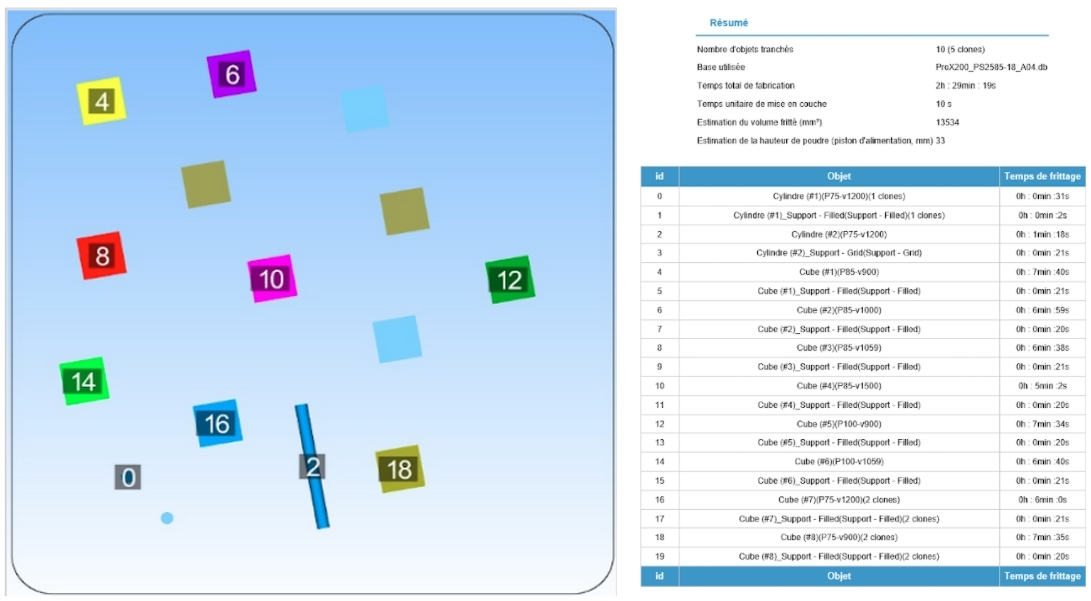
\includegraphics[scale=0.59]{Images/171024-cad}}
\decoRule
\caption[Specimens positions, order of fabrication and sintering times for batch X200-171024]{Specimens positions, order of fabrication and sintering times for batch X200-171024}
\label{fig:171024-cad}
\end{figure}

\begin{figure}[h!]
\centering
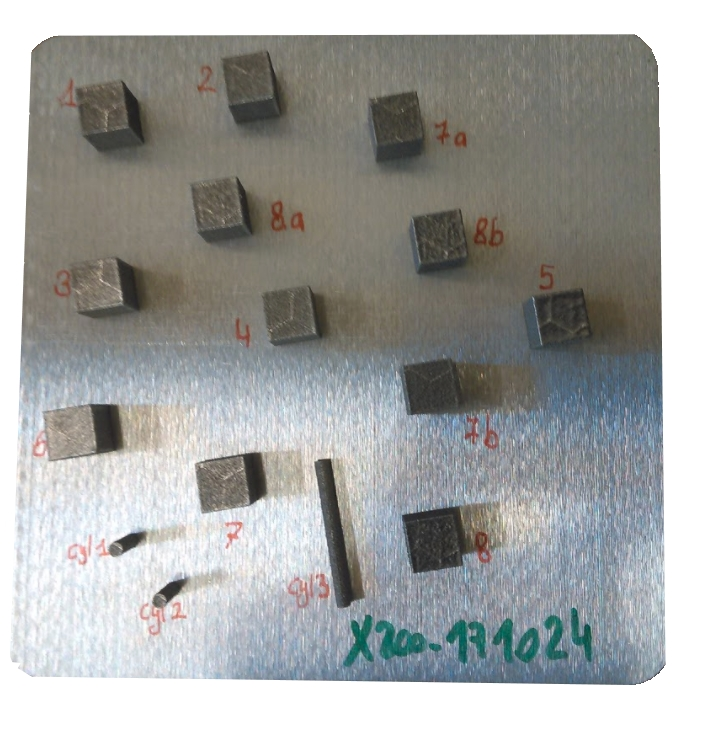
\includegraphics[scale=0.42]{Images/171024-real}
\decoRule
\caption[Photography of the manufacturing plate after completion of the fabrication of batch X200-171024]{Photography of the manufacturing plate after completion of the fabrication of batch X200-171024}
\label{fig:171024-real}
\end{figure}

\newpage
\subsection{Batch X200-180109}

\begin{figure}[ht]
\centering
\noindent\makebox[\textwidth]{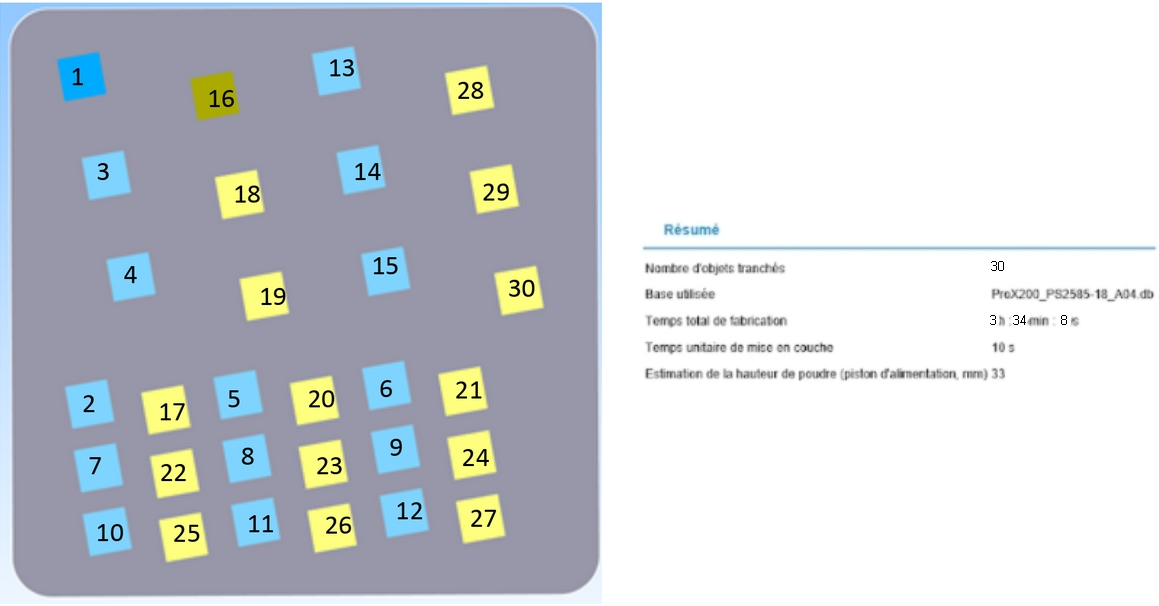
\includegraphics[scale=0.58]{Images/180109-cad}}
\decoRule
\caption[Specimens positions, order of fabrication and sintering times for batch X200-180109]{Specimens positions, order of fabrication and sintering times for batch X200-180109}
\label{fig:171024-cad}
\end{figure}

\begin{figure}[h!]
\centering
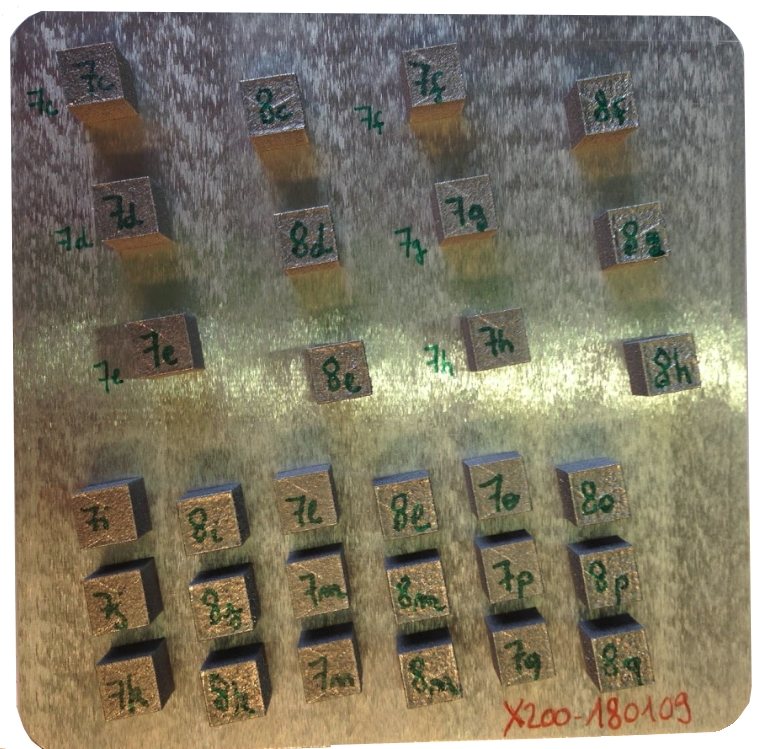
\includegraphics[scale=0.45]{Images/180109-real}
\decoRule
\caption[Photography of the manufacturing plate after completion of the fabrication of batch X200-180109]{Photography of the manufacturing plate after completion of the fabrication of batch X200-180109}
\label{fig:180109-real}
\end{figure}

\newpage
\subsection{Batch X200-180220}
\begin{figure}[h]
\centering
\noindent\makebox[\textwidth]{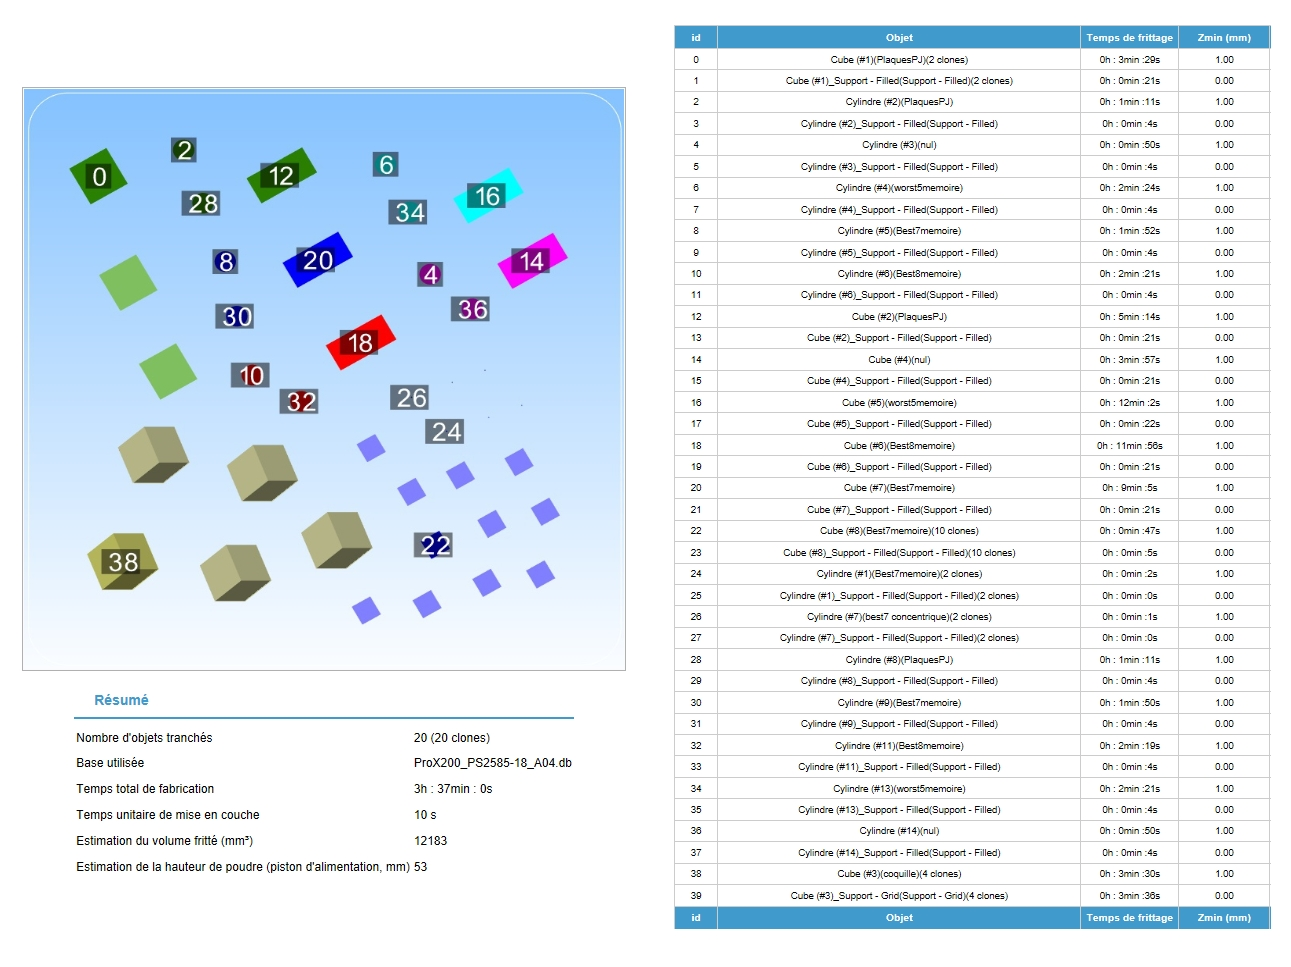
\includegraphics[scale=0.48]{Images/180220-cad}}
\decoRule
\caption[Specimens positions, order of fabrication and sintering times for batch X200-180220]{Specimens positions, order of fabrication and sintering times for batch X200-180220}
\label{fig:180220-cad}
\end{figure}